%!TEX root = ../../Main.tex
\graphicspath{{Chapters/Struktur/}}
%-------------------------------------------------------------------------------

\section{Struktur}

\subsection{BlackFin blokforklaring}

I dette projekt er der taget et valg udfra læringsmålene om at vi bruger Blackfin platformen til at udføre projektetes funktionalitet. Da en blackfin processor er bygget op af mange funktionalle blokke, vil der i det kommende afsnit laves et overblik over de interne forbindelser mellem hardware blokkene som bliver brugt i dette projekt. \cite{Struktur}

\begin{figure}[H]
	\centering
	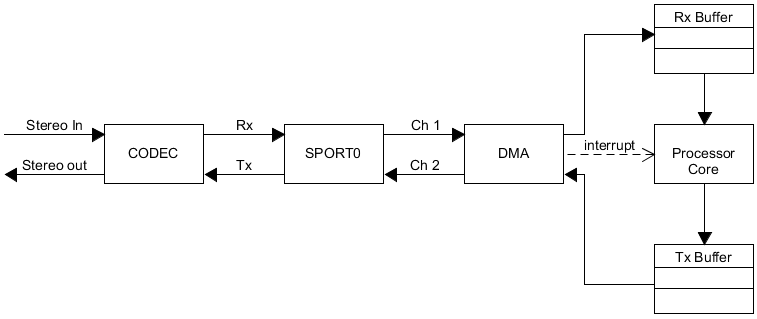
\includegraphics[width = 400pt]{Img/Struktur}
	\caption{Struktur NSS}
	\label{fig:Struktur}
\end{figure}

Igennem processen af vores funktionalitet, sendes lydsignalet gennem en codec1836, som har til opgave at sende inputtet gennem en ADC, hvorefter den sender det digitale signal videre til SPORT0, som står for at modtage og sende dataen. \\

DMA'en står for at sende dataen videre til Rx bufferen, når bufferen er fuld sender DMA'en interrupt til processeren om at procesere den modtagne data. \\
I den modsatte retning bliver det proceserede data flyttet til Tx bufferen, når Tx bufferen er fuld, sendes det til SPORT0 via DMA'en med Ch 2.  
Til sidst bliver dataen samplet gennem CODEC, som konverterer til et analogt signal vha. en DAC.
De forskellige blokke i strukturen fra figur \ref{fig:Struktur}, er implementeret i Init.C. 
  

\newpage

\subsection{Software arkitektur}
Til dette projekt har det været muligt at benytte et udleveret framework til Crosscore. Dette framework er lavet af Kim Bjerge, og er blevet modificeret af gruppen, til at virke med vores LMS filter. På \autoref{fig:Class diagram} kan man se hvilke klasser der er med i projektet og deres relationer til hinanden. 


\begin{figure}[H]
	\centering
	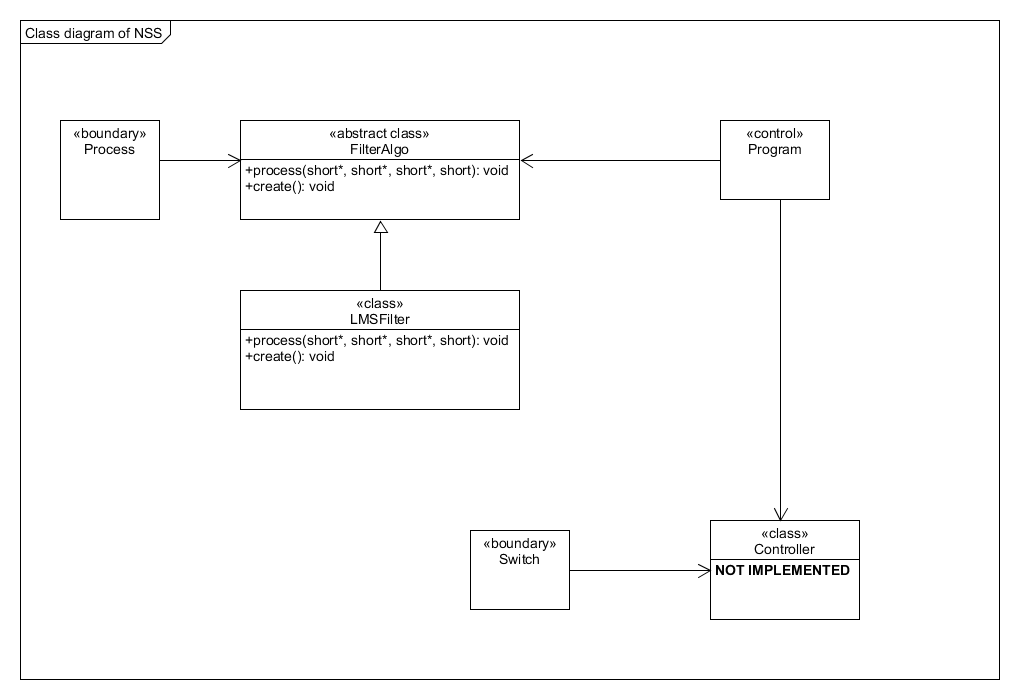
\includegraphics[width = 400pt]{Img/ClassDiagram.png}
	\caption{Klassediagram over NSS}
	\label{fig:Class diagram}
\end{figure}

Arkitekturen består af en abstrakt klasse FilterAlgo som har to virtuelle funktioner, process() og create(). Disse to nedarves af LMSFilter klassen og implementeres heri. Create() opretter filteret og nulstiller alle koefficienter, udover den første filter-koefficient, som bliver sat til 1. Grunden til dette er for at få det fulde støjsignal igennem første gang filteret kører. Dette vil blive uddybet mere i diskusion afsnittet. process() funktionen står for at filtrere uønsket støj fra tale signalet(d(n)). Koden er lavet så den følger vores matlab model så godt som overhovedet muligt. 

Vi har valgt ikke at implementere controller klassen, da vores 1. prioritet har været at få et fungerende LMS filter. Derfor står den som "NOT IMPLEMENTED". Istedet for at brugeren kan tænde for filteret med en switch, har vi valgt at lade filteret være aktiv så snart man starter programmet. 



\newpage


\begin{lstlisting}
for(short i = 0; i < len; i++)
{
	long fract yn = 0;

	for(short j = 0; j < NUM_WEIGTHS; j++)
	{
		if(i > j)
		{
			yn = yn + Filter.W[j]*x[i-j];
		}
	}
	y[i] = (fract)yn;
	e[i] = d[i] - yn;
		
	long fract tmp_W = 0;
		
	for(short k = 0; k < NUM_WEIGTHS; k++)
	{
		if(i > k)
		{
			Filter.W[k] = Filter.W[k]  + my*x[i-k]*e[i];
		}
	}
}
\end{lstlisting}

Koden ovenfor består af tre for-løkker. Den yderste løkke særger for at køre længden af signalet igennem. Løkken i linje 5, filtrere støjen så vi får vores støjsignal y(n). Dette støjsignal trækkes fra vores talesignal hvilket efterlader vores ønsket talesignal uden støj. Den sidste løkke på linje 17, opdaterer filter-koefficienterne så de hele tiden passer til støjen.

For at forsimple koden har vi valgt at splitte vores stereo kanal op i to, så det er muligt at få støjsignalet(x(n)) ind på højre kanal og tale signal(d(n)) ind på venstre kanal.


\begin{figure}[H]
	\centering
	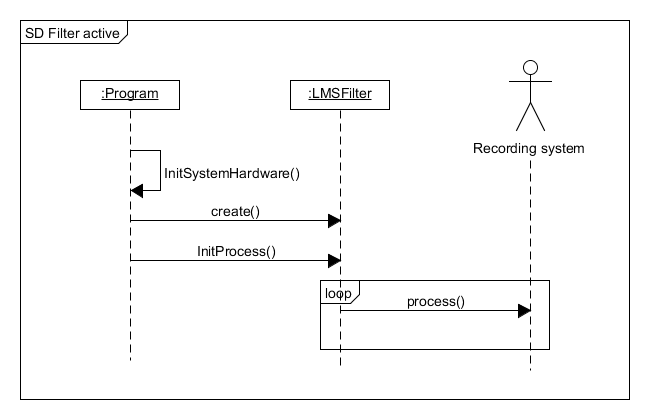
\includegraphics[width = 400pt]{Img/SD_filter_active.png}
	\caption{SD filter startes}
	\label{fig:SD}
\end{figure}
På sekvensdiagrammet nedenunder, kan man se hvordan koden køres igennem når filteret aktiveres. Process kører så længe systemet er aktivt, filtrerer uønsket støj fra og sender filtreret samples videre ud i systemet kontinuert.
